\begin{frame}{Mixnet}
    \centering
    \begin{figure}
        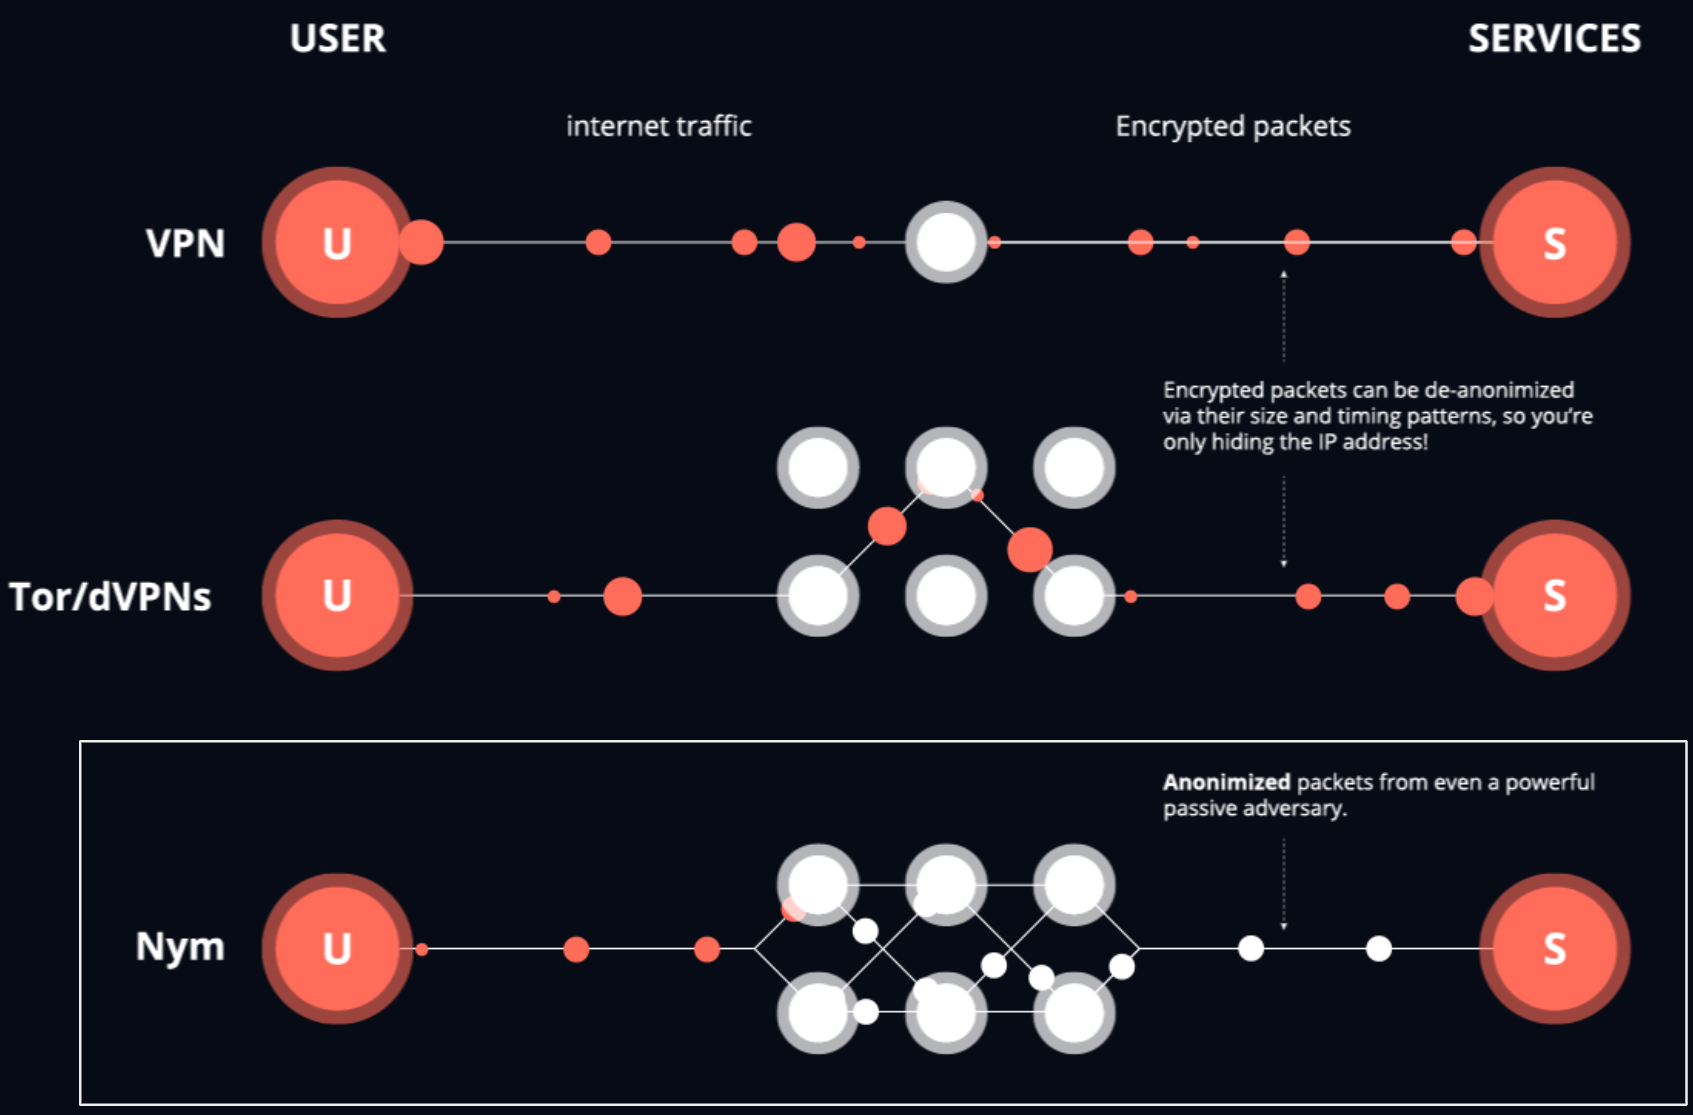
\includegraphics[width=0.8\linewidth]{Images/mixnet.png}
    \end{figure} 
\end{frame}

\begin{frame}{Schema overview}
    \centering
    \begin{figure}
        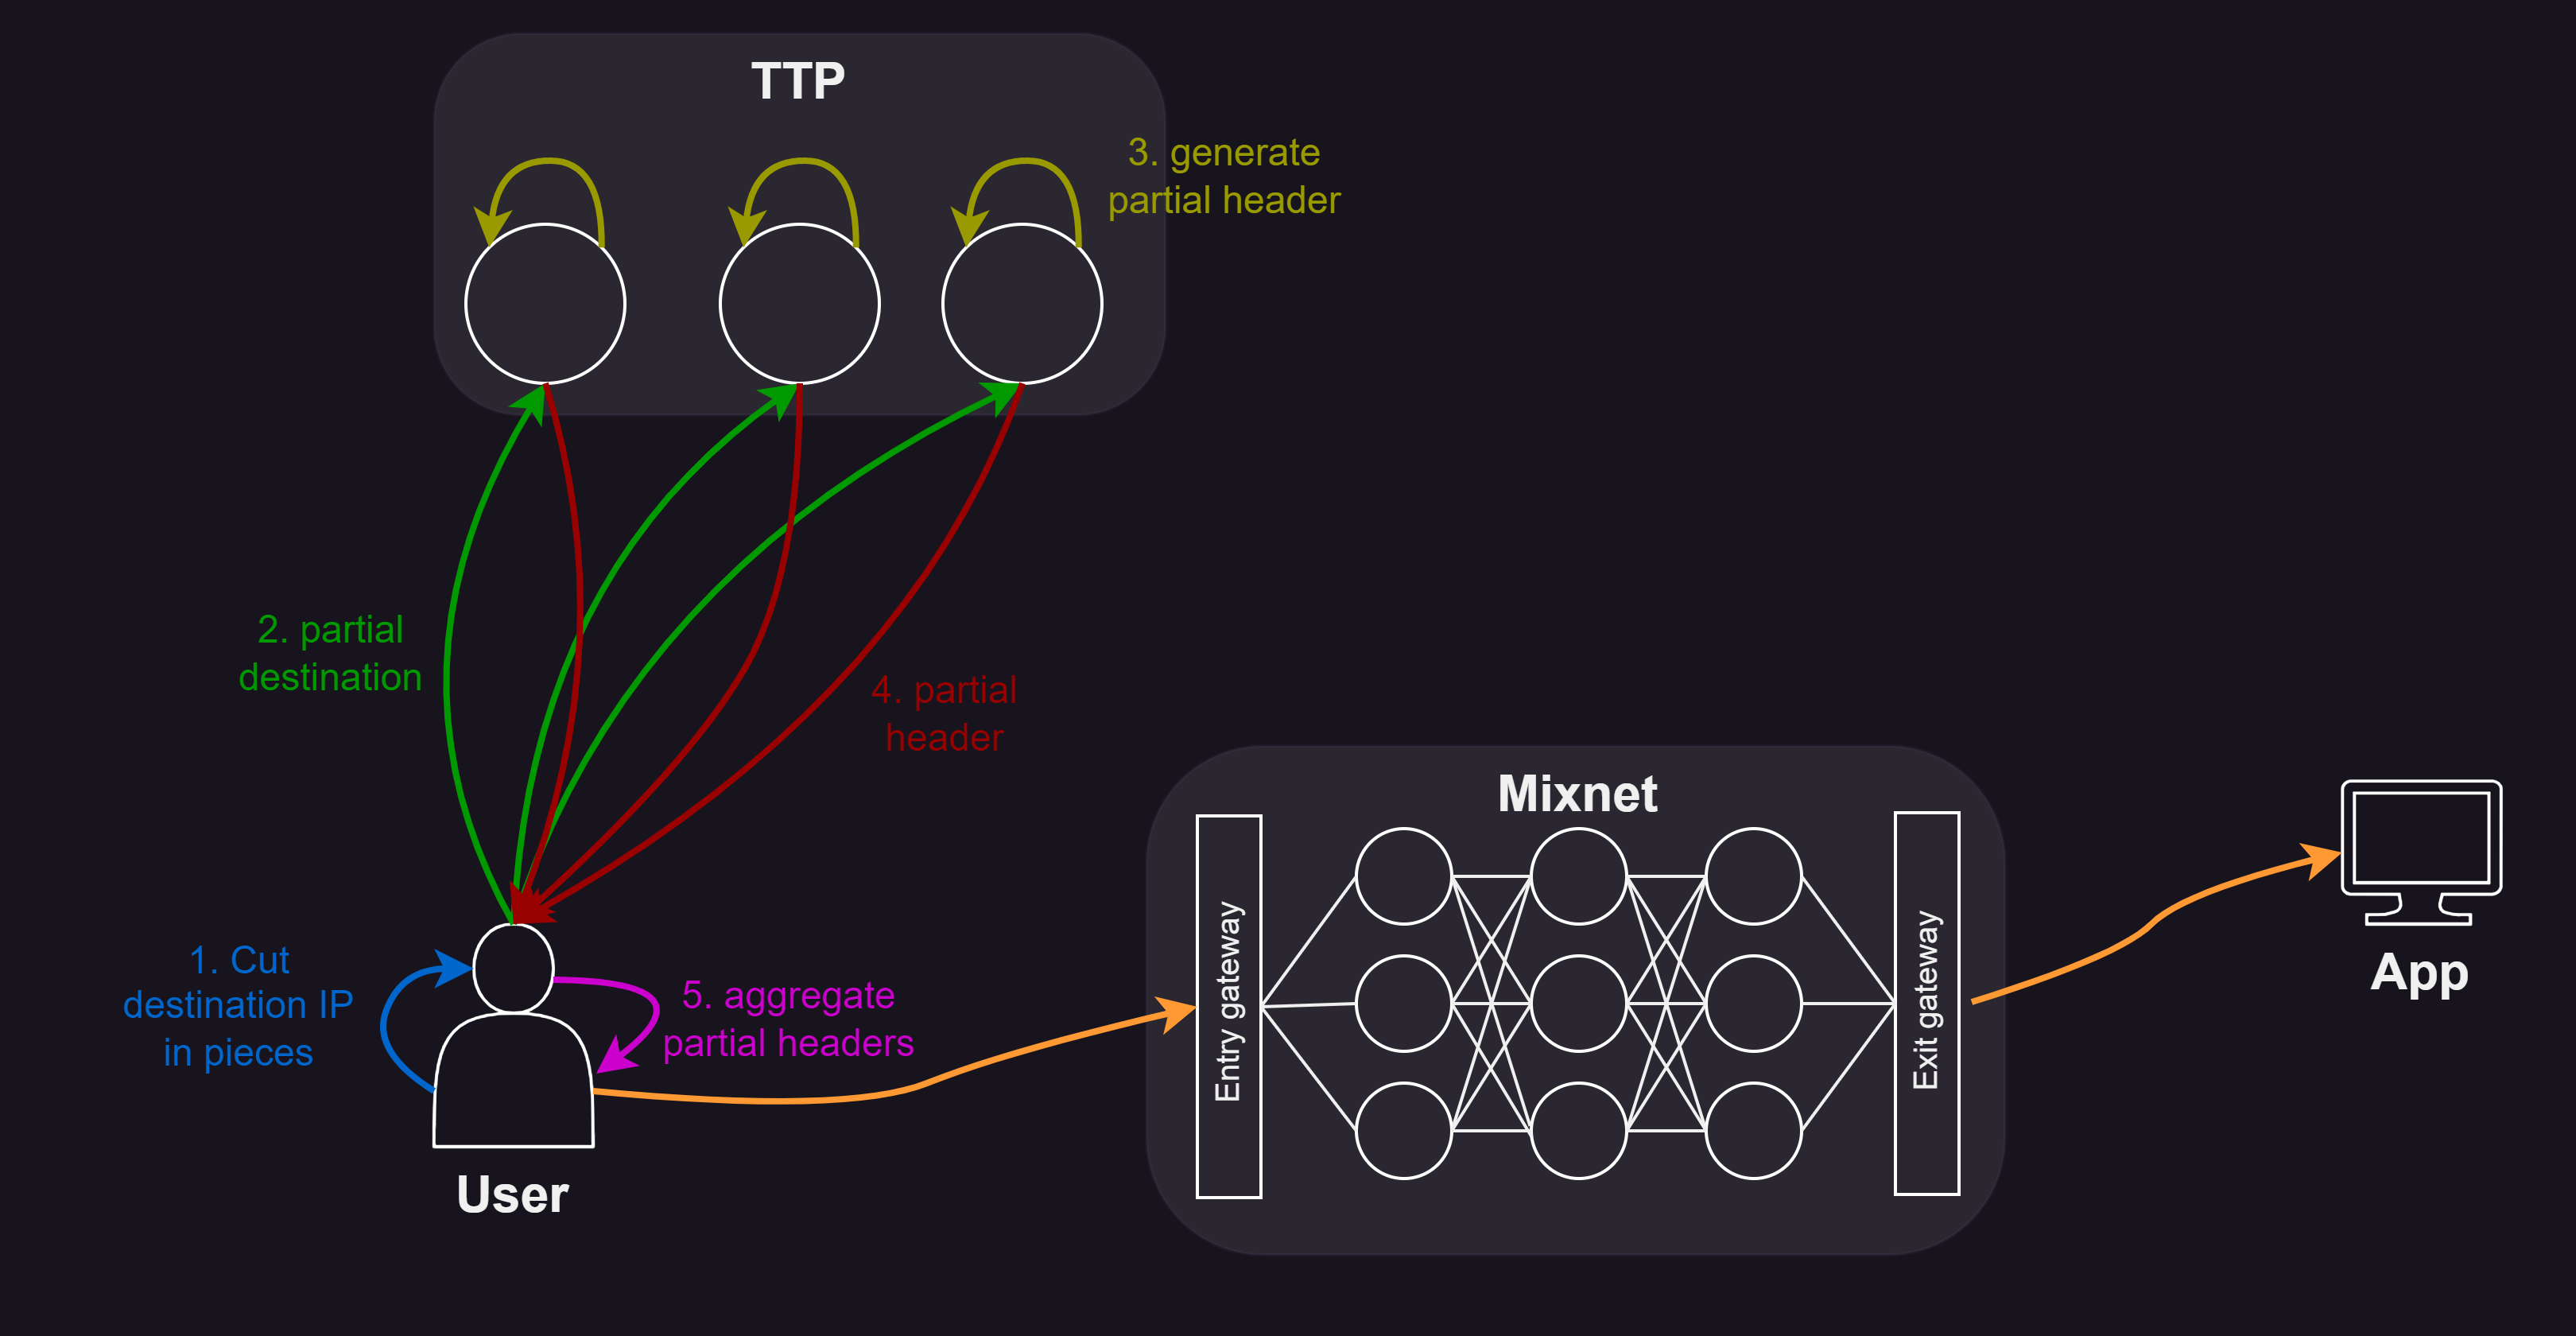
\includegraphics[width=\linewidth]{Images/sphinx_ttp.png}
    \end{figure}
\end{frame}

\begin{frame}{Desired properties}
    \begin{itemize}
        \setlength\itemsep{4mm}
        \onslide<1->
        \item {\normalsize Generic properties}
        \begin{itemize}
            \setlength\itemsep{2mm}
            \item {\color{lightgray}\textbf{\normalsize Correctness}: schema works without adversary}
            \item {\color{lightgray}\textbf{\normalsize Compactness}: Minimal overhead}
            \item {\color{lightgray}\textbf{\normalsize Efficiency}: Easy and fast to compute (e.g. XOR, hash, exponentiation,...)}
        \end{itemize}
        \onslide<2->
        \item {\normalsize Depends on the mixnode}
        \begin{itemize}
            \setlength\itemsep{2mm}\item {\color{olive}\textbf{\normalsize Forward / reply Undistinguishibility}: Cannot distinguish forward from reply packet}
            \item {\color{olive}\textbf{\normalsize Replay attack resistant:}: Cannot reused previous packet}    
        \end{itemize}
        \onslide<3->
        \item {\normalsize Depends on the header}
        \begin{itemize}
            \setlength\itemsep{2mm}
            \item {\color{olive}\textbf{\normalsize Integrity}: Maximum size path}
            \item {\color{orange}\textbf{\normalsize Wrap-resistance}: Unable to increase the intial path}
            \item {\color{red}\textbf{\normalsize Unlinkability}: Cannot link incoming and outgoing packet from a mixnode}
        \end{itemize}
    \end{itemize}
\end{frame}

\begin{frame}{Unlinkability compromised}
\begin{columns}
    \begin{column}{0.5\textwidth}
        \centering
        \vfill
        {\textbf{Original schema}}
        \vfill
        \begin{figure}
            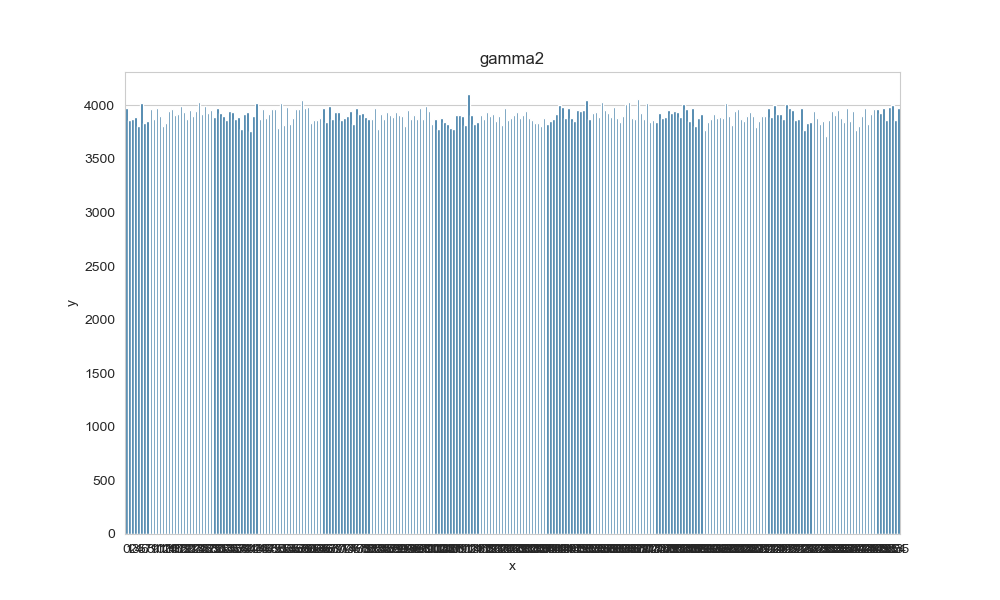
\includegraphics[scale=0.3]{Images/res/origin_gamma2.png}
        \end{figure}
    \end{column} 
    \vrule
    \begin{column}{0.5\textwidth}
        \centering
        \vfill
        {\textbf{My schema}}
        \vfill
        \begin{figure}
            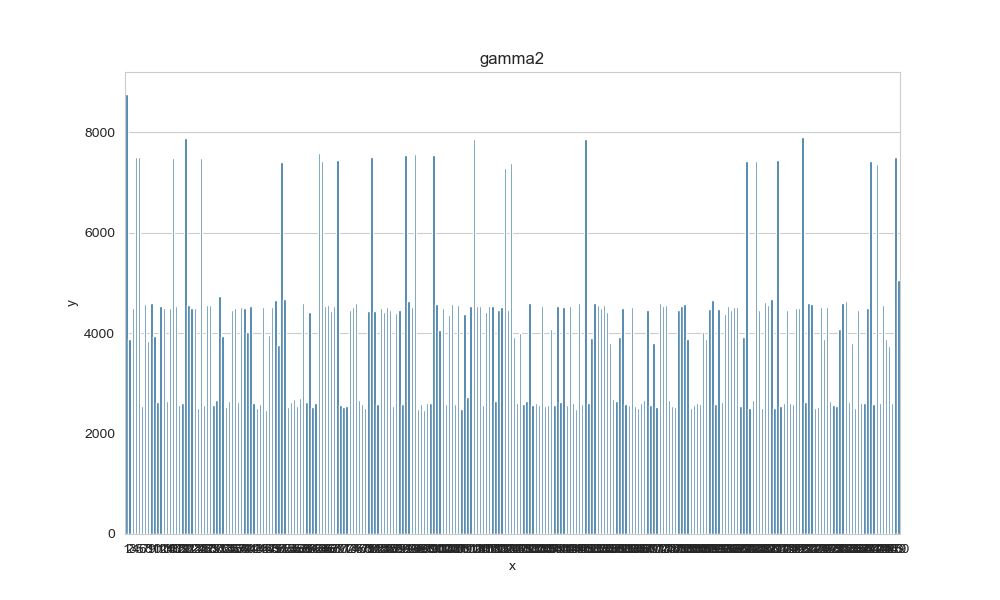
\includegraphics[scale=0.3]{Images/res/test_gamma2.png}
        \end{figure}
    \end{column}
\end{columns}
\end{frame}

\begin{frame}{Unlinkability compromised}
\centering
\begin{tikzpicture}
    \node (b1) [block=5]  at (2*\width, 0) {};
    \node (n1) [block=1]  at (0, 0) {$n_1$}; 
    \node (y1) [block=1]  at (\width, 0) {$\gamma_1$}; 
    \node [block=1] at (2*\width, 0) {$n_2$}; 
    \node [block=1] at (3*\width, 0) {$\gamma_2$}; 
    \node [block=1] at (4*\width, 0) {$n_3$}; 
    \node [block=1] at (5*\width, 0) {$\gamma_3$}; 
    \node [block=1, color=red] at (6*\width, 0) {$IP$};
\end{tikzpicture}
\begin{figure}
    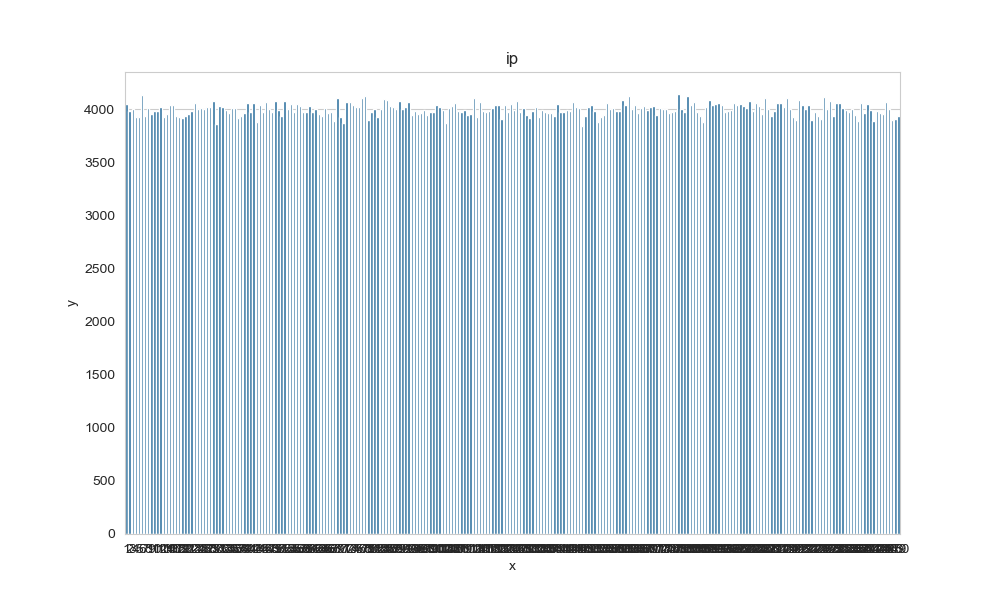
\includegraphics[width=0.9\linewidth]{Images/res/test_ip.png}
\end{figure}
\end{frame}

\begin{frame}{Unlinkability compromised}
    \centering
    \begin{tikzpicture}
        \node (b1) [block=5]  at (2*\width, 0) {};
        \node (n1) [block=1]  at (0, 0) {$n_1$}; 
        \node (y1) [block=1]  at (\width, 0) {$\gamma_1$}; 
        \node [block=1] at (2*\width, 0) {$n_2$}; 
        \node [block=1] at (3*\width, 0) {$\gamma_2$}; 
        \node [block=1] at (4*\width, 0) {$n_3$}; 
        \node [block=1, color=red] at (5*\width, 0) {$\gamma_3$}; 
        \node [block=1] at (6*\width, 0) {$IP$};
    \end{tikzpicture}
    \begin{figure}
        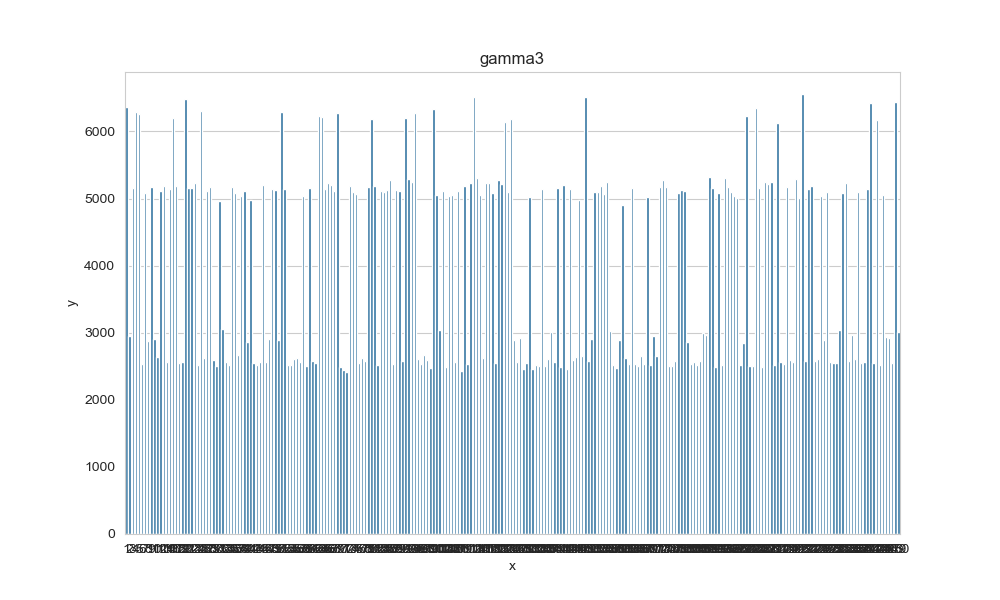
\includegraphics[width=0.9\linewidth]{Images/res/test_gamma3.png}
    \end{figure}
\end{frame}

\begin{frame}{Unlinkability compromised}
    \centering
    \begin{tikzpicture}
        \node (b1) [block=5]  at (2*\width, 0) {};
        \node (n1) [block=1]  at (0, 0) {$n_1$}; 
        \node (y1) [block=1]  at (\width, 0) {$\gamma_1$}; 
        \node [block=1] at (2*\width, 0) {$n_2$}; 
        \node [block=1] at (3*\width, 0) {$\gamma_2$}; 
        \node [block=1, color=red] at (4*\width, 0) {$n_3$}; 
        \node [block=1] at (5*\width, 0) {$\gamma_3$}; 
        \node [block=1] at (6*\width, 0) {$IP$};
    \end{tikzpicture}
    \begin{figure}
        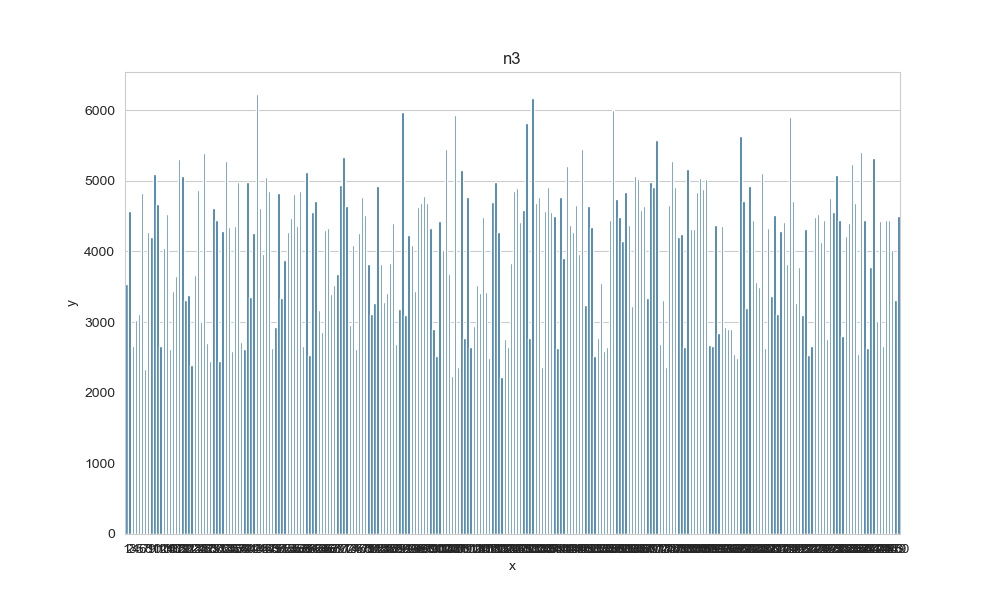
\includegraphics[width=0.9\linewidth]{Images/res/test_n3.png}
    \end{figure}
\end{frame}

\begin{frame}{Unlinkability compromised}
    \centering
    \begin{tikzpicture}
        \node (b1) [block=5]  at (2*\width, 0) {};
        \node (n1) [block=1]  at (0, 0) {$n_1$}; 
        \node (y1) [block=1]  at (\width, 0) {$\gamma_1$}; 
        \node [block=1] at (2*\width, 0) {$n_2$}; 
        \node [block=1, color=red] at (3*\width, 0) {$\gamma_2$}; 
        \node [block=1] at (4*\width, 0) {$n_3$}; 
        \node [block=1] at (5*\width, 0) {$\gamma_3$}; 
        \node [block=1] at (6*\width, 0) {$IP$};
    \end{tikzpicture}
    \begin{figure}
        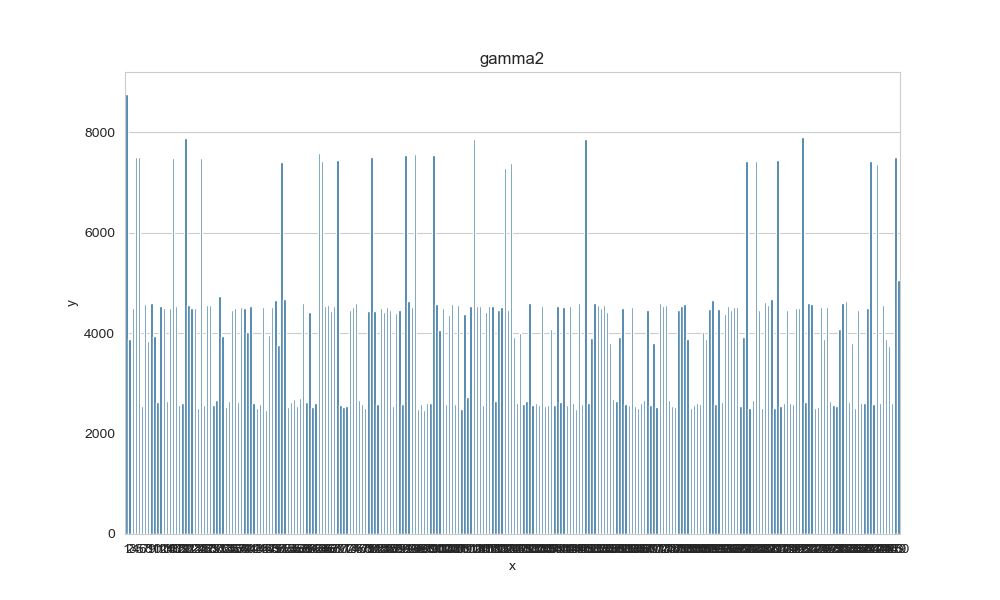
\includegraphics[width=0.9\linewidth]{Images/res/test_gamma2.png}
    \end{figure}
\end{frame}

\begin{frame}{Unlinkability compromised}
    \centering
    \begin{tikzpicture}
        \node (b1) [block=5]  at (2*\width, 0) {};
        \node (n1) [block=1]  at (0, 0) {$n_1$}; 
        \node (y1) [block=1]  at (\width, 0) {$\gamma_1$}; 
        \node [block=1, color=red] at (2*\width, 0) {$n_2$}; 
        \node [block=1] at (3*\width, 0) {$\gamma_2$}; 
        \node [block=1] at (4*\width, 0) {$n_3$}; 
        \node [block=1] at (5*\width, 0) {$\gamma_3$}; 
        \node [block=1] at (6*\width, 0) {$IP$};
    \end{tikzpicture}
    \begin{figure}
        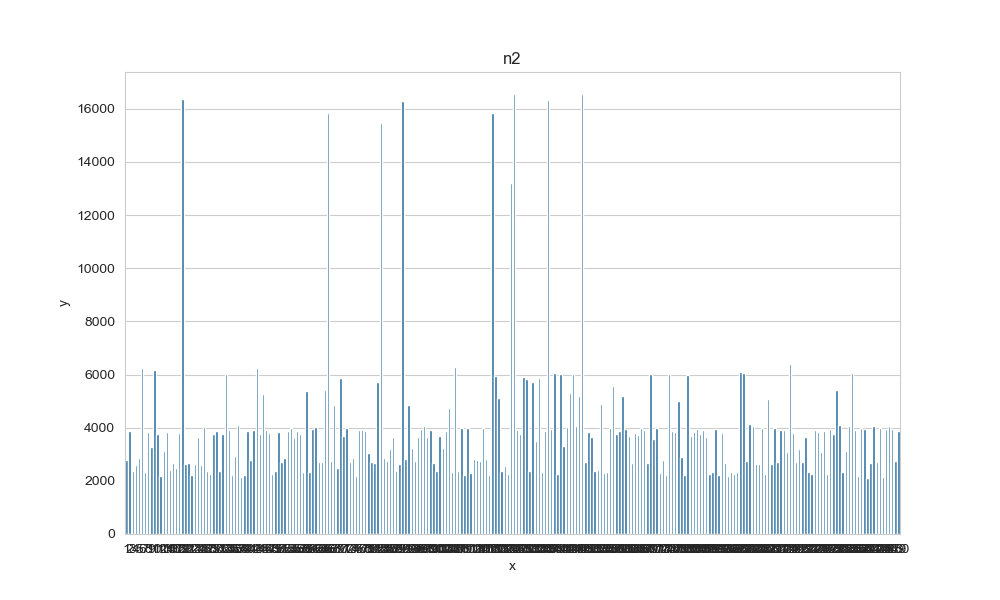
\includegraphics[width=0.9\linewidth]{Images/res/test_n2.png}
    \end{figure}
\end{frame}

\begin{frame}{Unlinkability compromised}
    \centering
    \begin{tikzpicture}
        \node (b1) [block=5]  at (2*\width, 0) {};
        \node (n1) [block=1]  at (0, 0) {$n_1$}; 
        \node (y1) [block=1, color=red]  at (\width, 0) {$\gamma_1$}; 
        \node [block=1] at (2*\width, 0) {$n_2$}; 
        \node [block=1] at (3*\width, 0) {$\gamma_2$}; 
        \node [block=1] at (4*\width, 0) {$n_3$}; 
        \node [block=1] at (5*\width, 0) {$\gamma_3$}; 
        \node [block=1] at (6*\width, 0) {$IP$};
    \end{tikzpicture}
    \begin{figure}
        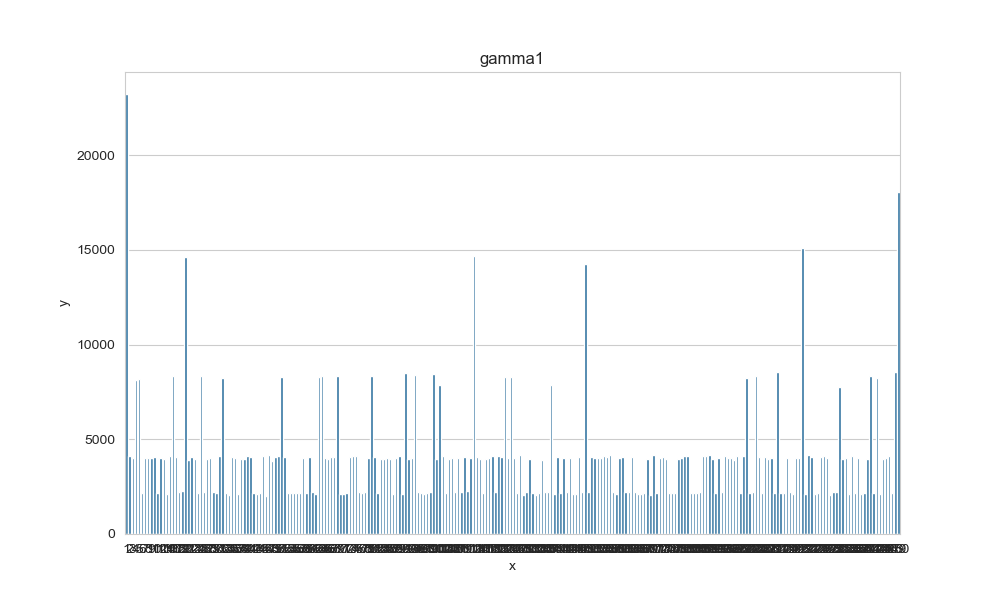
\includegraphics[width=0.9\linewidth]{Images/res/test_gamma1.png}
    \end{figure}
\end{frame}

\begin{frame}{Unlinkability compromised}
    \centering
    \begin{tikzpicture}
        \node (b1) [block=5]  at (2*\width, 0) {};
        \node (n1) [block=1, color=red]  at (0, 0) {$n_1$}; 
        \node (y1) [block=1]  at (\width, 0) {$\gamma_1$}; 
        \node [block=1] at (2*\width, 0) {$n_2$}; 
        \node [block=1] at (3*\width, 0) {$\gamma_2$}; 
        \node [block=1] at (4*\width, 0) {$n_3$}; 
        \node [block=1] at (5*\width, 0) {$\gamma_3$}; 
        \node [block=1] at (6*\width, 0) {$IP$};
    \end{tikzpicture}
    \begin{figure}
        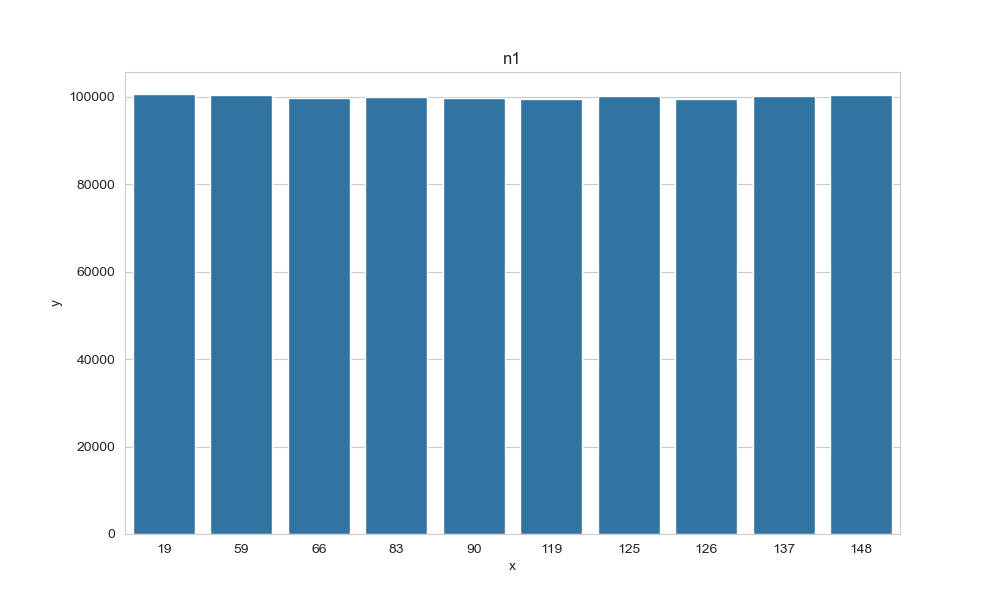
\includegraphics[width=0.9\linewidth]{Images/res/test_n1.png}
    \end{figure}
\end{frame}